\documentclass[letterpaper,10pt,draftclsnofoot,onecolumn,titlepage]{IEEEtran}

\usepackage{graphicx}
\usepackage{amssymb}
\usepackage{amsmath}
\usepackage{amsthm}
\usepackage{alltt}
\usepackage{float}
\usepackage{color}
\usepackage{url}
\usepackage{enumitem}
\usepackage{pstricks, pst-node}
\usepackage{geometry}
\usepackage{array}


\geometry{margin = .75in}

\usepackage{hyperref}



\newcommand*{\signature}[1]{%
	\par\noindent\makebox[3.5in]{\hrulefill} \hfill\makebox[3.0in]{\hrulefill}%
	\par\noindent\makebox[3.5in][l]{#1}	    \hfill\makebox[3.0in][l]{Date}%
}%

\def\name{Kevin Stine, Courtney Bonn, Maxwell Dimm}
\def\team{Calvary Chapel Corvallis}
\def\grp{Group \#62}

\hypersetup{
	colorlinks = true,
	urlcolor = black,
	linkcolor = black,
	pdfauthor = {\name},
	pdftitle = {CS461 Design Document},
	pdfsubject = {CS461 Design Document},
	pdfpagemode = UseNone
}

\begin{document}
	\title{\huge \team \\ Design Document \\ CS 461 Fall 2016}
	\author{\large \name \\ \grp}



	\maketitle


		\begin{abstract}The purpose of this project is to produce an iOS/Android application for Calvary Chapel of Corvallis that will allow members to access a plethora of information all in one localized space.
		The Church's current website does not provide an interface where current members of the church can very quickly access important information such as events, bulletins, and messages from the service.
		The desired application will be simple enough for anyone to use while providing back end access for staff to easily upload new information to the app.
		The priorities lie in maximizing the usability of the app and providing bulletin, schedule, video, and giving functionality.
		We will work with the existing Calvary Chapel web development team to create a product that is seamlessly integrated with their already existing network.
		\end{abstract}


	\clearpage

	\tableofcontents

	\clearpage

	\section{Overview}

		\subsection{Scope}
			We will be implementing a mobile application for both iOS and Android platforms.
			This app will provide the members of Calvary Chapel Corvallis a centralized hub that will allow them to access the most important information about the church.
			Users will be able to view announcements, a calendar, e-bulletins, and sermons.
			Users will also be able to donate to the church.
			Three people will be involved in the implementation of this software and it will be done during October 2016 and June 2017.

		\subsection{Purpose}
			The purpose of this design document is to detail how the application software will be designed.
			We will discuss how we will meet the requirements for our church application and discuss the structure of the application.
		\subsection{Intended Audience}
			The intended audience of this design document will be our clients, the teachers of CS 461, as well as the teacher's assistants.


	\section{Definitions}
		\begin{itemize}
			\item \textbf{Model-View-Controller:} A design pattern that assigns objects in an application one of three roles: model, view, or controller. Also called MVC.
		\end{itemize}


	\section{Conceptual model for software design descriptions}

		\subsection{Software design in context}

		\subsection{Software design descriptions within the life cycle}

			\subsubsection{Influences on SDD preparation}
				The key influence on this software design document is the software requirements specification document (SRS) that has previously been documented.
				The requirements listed in the SRS will greatly determine the design of the software and how we implement this project.

			\subsubsection{Influences on software life cycle products}
				This software design document may lead to necessary changes in the SRS.
				Throughout development, it's possible that there will be design changes that require us to change details in the SRS.
				Testing may also be changed based on the design document.

			\subsubsection{Design verification and design role in validation}
				In order to determine if the application has met requirements, we will perform user testing.
				This will involve having users try to use the software in the intended manner and see if they are successful.
				Success will be determined by how many users are successfully able to use the application without errors or issues.

	\section{Design description information content}

		\subsection{Introduction}
			Within this design document, there are many required contents.
			We will identify the software design document and it's stakeholders.
			We will discuss design concerns and selected design viewpoints.
			We will also discuss design views, design overlays, and the design rationale.

		\subsection{SDD Identification}
			A valid software design document includes the following parts:
			\begin{itemize}
				\item{Date of issue and status}
				\item{Scope}
				\item{Issuing organization}
				\item{Authorship}
				\item{References}
				\item{Context}
				\item{One or more design languages for each design viewpoint used}
				\item{Body}
				\item{Summary}
				\item{Glossary}
				\item{Change history}
			\end{itemize}

		\subsection{Design stakeholders and their concerns}
			The design stakeholders of the Calvary Chapel of Corvallis application are the developers of the app and the team at the church.
			Design concerns of the stakeholders include creating an application that is user-friendly and very simplistic in design features.
			The final application will be designed in a way that will ease this concern, as the intended design will be a very easy-to-use application.

		\subsection{Design views}
		We will use Unified Model Language (UML) diagrams in order to describe and represent the views of our system.

		\subsection{Design viewpoints}
		There are many viewpoints that will be covered in this document including: context, composition, logical, dependency, and interaction viewpoints.
		They each mean different things, for example the context viewpoint will cover what type of users will be using the app and the perceptions they should have over it.
		The composition viewpoint will cover what information and content will be hosted within the app.
		The logical viewpoint will cover what purpose the app will serve and how it will accomplish those purposes.
		Dependency will be the things the app needs in order for it to work as designed and the integration of it with other applications.
		Finally, we will conclude with the interaction viewpoint witch will cover how people will use our app and how it will interact with various other technologies.

		\subsection{Design elements}

		\subsection{Design overlays}

		\subsection{Design rationale}
		Two of the primary focuses in our design rationale are to keep it simple for the users, and to keep is simple for the church management team.
		The client wants the app to be as user friendly for the congregation at possible, along with keeping the back end work to a minimum.
		If the app is too confusing for the users or the team, then the whole purpose of this app will be voided by their inability to use it.
		Secondary to these points is maximizing speed and adding additional small features.
		We should be creating an efficient app that can have helpful functionality for the users.

		\subsection{Design languages}
		The design language that we will use in this document will be UML.

	\section{Design Viewpoints}

		\subsection{Introduction}
		In this section, we will discuss seven design viewpoints including:
			\begin{itemize}
				\item{Context Viewpoint}
				\item{Composition Viewpoint}
				\item{Logical Viewpoint}
				\item{Dependency Viewpoint}
				\item{Patterns Use Viewpoint}
				\item{Interface Viewpoint}
				\item{Interaction Viewpoint}
			\end{itemize}

		\subsection{Context Viewpoint}
		Included in the app are four primary functionalities: calendar, sermons, donations, and bulletin.
		The reason being is that these are the four primary things that our client believes their users will be looking to access from the app.
		The schedule will be there to allow users to see what is going on within the church in the long-term.
		The sermon functionality will allow people to view past sermons in case they missed them or simply want to recap a message they enjoyed.
		In this church and many others donating is a major part of what they do.
		Making this easier for the users of our app is crucial.
		Now they can do it from home or any time because the app will allow them to give without the need of cash on hand.
		Finally the last functionality that we want to include is the bulletin.
		This will be a place for the users to grab quick info that would normally be handed out on a piece of paper inside the building.
		his will allow them to view the bulletin from anywhere at any time and reduce costs for the church to prevent the need of printing off pamphlets.

		\begin{figure}[H]
			\centering
			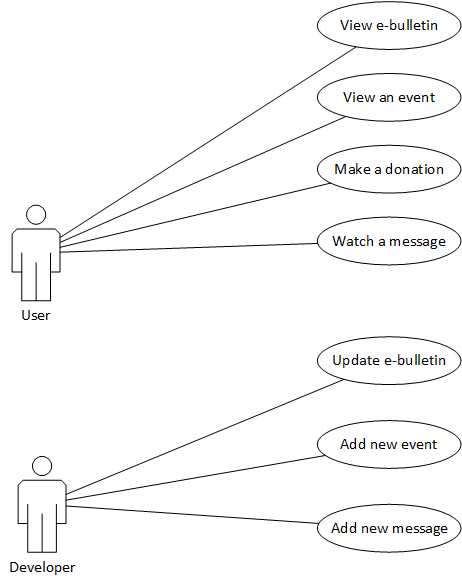
\includegraphics[natwidth=462, natheight=585]{UseCase.png}
			\caption{Use Case Diagram}
			\label{fig:usecase}
		\end{figure}

		\subsection{Composition Viewpoint}
			Our system is composed of four components which are an iOS Client, an Android Client, a Database Server and a Web Server.
			The Database Server which we connect to is through Church Community Builder.
			The Web Server which we connect to is Calvary Chapel's current website.
			Client components are comprised of smartphone applications, based on their operating system.
			Our iOS and Android Clients will be able to pull information from both CCB as well as the church's current website.

		\begin{figure}[H]
			\centering
			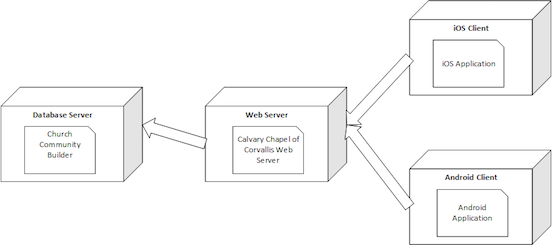
\includegraphics[natwidth=552, natheight=245]{Deployment.png}
			\caption{Deployment Diagram}
			\label{fig:deployment}
		\end{figure}

		\subsection{Logical Viewpoint}

		\subsection{Dependency Viewpoint}
			The app will have a couple interconnections with other apps/plugins.
			The first and foremost will be with church community builder.
			Most of the information we will be pulling from continuously will be from CCB, such as the schedule and bulletin.
			Also we will need to work with livestreams API to get a functional video/audio player for the sermons section.
			Our client already uses foxycart for their donation service so we will integrate their service to our app using their published API.
			We will be sending information to their servers so we will also need to find a way to encrypt the data being sent because it is highly personal info.

		\subsection{Patterns use viewpoint}
			Our system will make use of the Model-View-Controller (MVC) design pattern.
			The MVC design pattern assigns objects in an application with one of three roles: model, view or controller.
			In addition to defining the roles the objects play in the application, it also defines the way objects communicate with each other.
			For example when the user refreshes the sermons page to get the latest sermons, the model object changes and notifies the controller object which will then update the sermons view objects.

			\subsubsection{Model Objects}
				Model objects encapsulate the data specific to the application and define the logic and computation that manipulate and process the data.
				In our application, there will be data specific to donations, calendar, e-bulletins and messages.
				This will strictly be the data that we pull from the CCB database and the Church's website and will not be concerned with user-interface and presentation issues.
				We will parse the CCB information as XML and read that into our application as XML.
				The model object will strictly deal with data pulled from the CCB database.
				Once the data has been retrieved, it will notify the controller object to begin the process of updating the user's view.
				This object is hidden via an abstraction layer, ensuring that the user is only able to view the information we provide them in a clean and concise view.

			\subsubsection{View Objects}
				The view object is an object in an application that the users can see.
				Our application will utilize the view objects to display data from our model object which is pulled from CCB.
				This object is what the user will see and interact with through our application.
				View objects will be consistent across pages to ensure the most navigable UI for the user.
				An example of the view object would be when the user wants to view the calendar for events.
				If they are in the month of December and want to look ahead to January, they will tap to proceed to the next month, which will notify the controller object letting the model object know to pull January's data from the database.

			\subsubsection{Controller Objects}
				The controller object will act as an intermediary between our applications views and its model objects.
				The controller will be a conduit through which view objects learn about changes in model objects and vice versa.
				In addition to communication between the view and model objects, the controller object will also perform setup, coordinate tasks and manage the life cycle of other objects.
				When the model object is updated with the month of January, the controller object communicates the new data to the view objects so they can be displayed to the user.


		\subsection{Interface viewpoint}
			The interface as stated above is planned to be simple.
			For navigation we will be using a sidebar most likely for both IOS and Android for continuity.
			For IOS we will be using interface builder to simplify the process of designing the layout and from there we will try to carry over a lot of the format to android keeping the design elements that make sense.
			The app will accept input in the form of clicking and text for the purpose of selections and donations respectively.
			We will pull banners and seasonal stylings from the client’s website to stay up-to-date with their webpage.
			The sermons functionality of the app will list different messages that were most recently uploaded on livestream.
			Once selected will automatically play from the livestream plugin we will integrate with the app.


		\subsection{Interaction Viewpoint}
			The Interaction viewpoint describes the high-level functionality of each part of the app.
			There are four different functionalities that will be addressed: viewing the calendar, reading the bulletin, donating to the church, and watching the message.

			\subsubsection{Viewing the Calendar}
				\begin{enumerate}
					\item \textbf{Open Application:} The interaction begins with the user open the iOS or Android application.
					\item \textbf{Click Calendar:} After opening the application, the user will see the menu and choose the option to view the calendar.
					\item \textbf{Pull Calendar:} Once the user has clicked on the calendar, the application will fetch the calendar from the database, Church Community Builder.
					\item \textbf{Return and Display Calendar:} The database will then display the calendar on the application.
				\end{enumerate}

			\subsubsection{Reading the Bulletin}
				\begin{enumerate}
					\item \textbf{Open Application:} The interaction begins with the user open the iOS or Android application.
					\item \textbf{Click Bulletin:} After opening the application, the user will see the menu and choose the option to open the bulletin.
					\item \textbf{Pull Bulletin:} Once the user has clicked on the bulletin, the application will fetch the e-bulletin from the database, Church Community Builder.
					\item \textbf{Return and Display Bulletin:} The database will then display the e-bulletin on the application.
				\end{enumerate}

			\subsubsection{Donating to the Church}
				\begin{enumerate}
					\item \textbf{Open Application:} The interaction begins with the user open the iOS or Android application.
					\item \textbf{Click Bulletin:} After opening the application, the user will see the menu and choose the option to donate.
					\item \textbf{Load Donation Page:} Once the user has clicked on the donate button, a page will load that will connect the user to Calvary Chapel of Corvallis' webpage that will display the donation page.
					The user will then follow the instructions on the page to continue making a donation to the church.
				\end{enumerate}

			\subsubsection{Watching the Message}
				\begin{enumerate}
					\item \textbf{Open Application:} The interaction begins with the user open the iOS or Android application.
					\item \textbf{Click Messages:} After opening the application, the user will see the menu and choose the option to open the messages.
					\item \textbf{Pull Messages:} Once the user has clicked on the messages, the application will fetch the message from LiveStream.
					\item \textbf{Return and Display Message:} LiveStream will then display the recent video message.
				\end{enumerate}




	\section{Conclusion}



\end{document}
